\documentclass[12pt, a4paper]{article}
\usepackage[utf8]{inputenc}
\usepackage[T1]{fontenc}
\usepackage[slovene]{babel}
\usepackage{lmodern}
\usepackage{amsmath}
\usepackage{units}
\usepackage{float}
\usepackage{eurosym}
\usepackage{amsfonts}
\usepackage{fancyhdr,amssymb,amsmath,amsthm,bbm,enumerate,mdwlist,url,multirow,hyperref,graphicx}
\usepackage{pdfpages}
\usepackage{comment}
\usepackage{breqn}

\usepackage{enumerate}
\setlength{\parindent}{0mm}

\DeclareUnicodeCharacter{2212}{-}

\begin{document}
\begin{titlepage}
\begin{center}

\large
Univerza v Ljubljani\\
\normalsize
Fakulteta za matematiko in fiziko\\

\vspace{5 cm} 

\large
Finančni praktikum \\


\vspace{0.5cm}
\LARGE
\textbf{Lokalno iregularno barvanje povezav}

\vspace{0.5 cm}

\large
Domen Flakus Bosilj in Lara Jagodnik \\


\vspace{1.5cm}
\normalsize
Mentorja: prof. dr. Riste Škrekovski, asist. dr. Janoš Vidali
\vspace{3cm}


\vfill

\large Ljubljana, 2020

\end{center}
\end{titlepage}


\newpage

\tableofcontents
\vspace{22mm}

\newpage

\section{Uvod}

V projektu pri finančnem praktikumu si bova ogledala lokalno iregularno barvanje povezav. Pri obravnavi problema bova delala z neusmerjenimi grafi. Projekt bova izdelala v programu Sage. \\
Graf $G$ je lokalno iregularen, če imata vsaki dve sosednji vozlišči $u$ in $v$ različno stopnjo, $deg(u) \neq deg(v)$. (Stopnja vozlišča nam pove število povezav, ki potekajo iz vozlišča.) \\
Barvanje povezav je lokalno iregularno, če vsaka barva inducira lokalno iregularen graf. \\
V projektu bova preverila ali drži domneva, da je vsak kubičen graf lokalno iregularno 3-obarvljiv. To pomeni, da lahko graf pobarvamo s tremi barvami tako, da razpade na tri lokalno iregularne grafe. (Kubični graf je graf v katerem imajo vsa vozlišča stopnjo 3.)\\


Lastnosti grafov, ki so povezani z najino temo:
\begin{itemize}

\item Poti lihe dolžine ne dopuščajo lokalno iregularnega barvanja.
\item Graf je ''decomposable'' če dopušča lokalno iregularno barvanje.
\item Najmanjši $k$ za katerega obstaja lokalno iregularno barvanje v grafu $G$ s $k$ barvami se imenuje lokalni iregularni kromatični indeks in ga označimo z $x^'_{irr}(G)$
\item Naj bo $G$ ''decomposable'' graf. Potem je $x^'_{irr}(G) \leq 328$.
\item Domneva, da je $x^'_{irr}(G) \leq 3$ je že dokazana za posebne vrste grafov, kjer je najmanjša stopnja vozlišč vsaj $10^{10}$ in za $k$-regularne grafe, kjer je $k \geq 10^7$.

\end{itemize}

\newpage
\section{Kaj sva delala in kako dela algoritem}\textit{}\textit{}

Problem sva najprej obravnavala na manjših grafih (do vključno 12 vozlišč), ki sva jih generirala s pomočjo funkcije graphs.nauty_geng. Ker pri tako majhnem številu vozlišč grafov še ni veliko, (kubičnih grafov na 10 vozliščij je 19, na 12 vozliščih pa 85) sva pregledala čisto vse možne.

Grafe sva naključno pobarvala, nato sva poiskala povezave, kjer se pojavi težava. Najprej sva nameravala v vsakem obhodu funkcije čez vse povezave in ob tem pogledati ali se barvo splača spremeniti. Ker sva ugotovila da tak algoritem na velikih grafih deluje zelo počasi, sva funkcijo randomizirala. Barvanje sva nato spreminjala tako, da sva za naključno  povezavo pogledala, ali sprememba barve te povezave morda zmanjša število povezav, ki ne ustrezajo pogoju lokalne iregularnosti grafa. Če je bilo barvanje neuspešno, sva na istem grafu poskusila začeti z novim drugačnim barvanjem in v najslabšem primeru to ponovila 10-krat.


\begin{figure}[H]
\centering
\begin{minipage}{.5\textwidth}
  \centering
  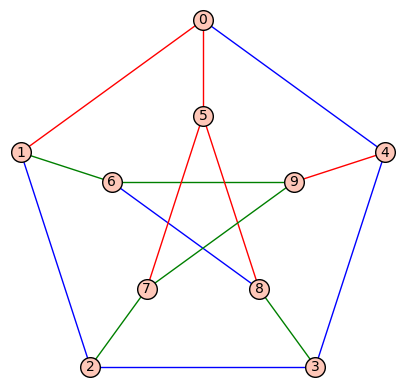
\includegraphics[width=.8\linewidth]{petersen_pred.png}
  \captionof{Naključno pobarvan Petersenov graf}
  \label{fig:naključno pobarvan Petersenov graf}
\end{minipage}%
\begin{minipage}{.5\textwidth}
  \centering
  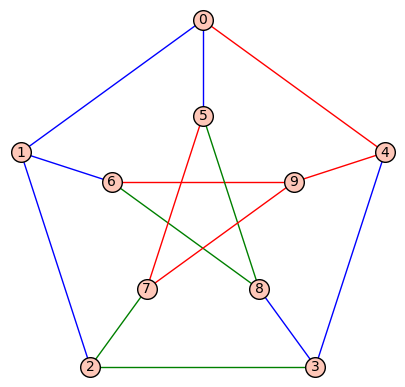
\includegraphics[width=.8\linewidth]{petersen_po.png}
  \captionof{Lokalno iregularno pobarvan $Petersenov$ $graf$}
  \label{fig:lokalno iregularno pobarvan $Petersenov$ $graf$}
\end{minipage}
\end{figure}

Za primer prikaza delovanja algoritma sva vzela najbolj znan kubičen graf na 10 vozliščih, to je $Petersenov$ $graf$. Na sliki 1 je prikazano naključno začetno barvanje, na sliki 2 pa koncno barvanje ki je lokalno iregularno.

Nato sva konstruirala naključne ”velike” kubične grafe z graphs.RandomRegular, na vozliščih 14, 16, 18, 20 in število vozlišč večala za 10 do 70. Tu nisva pregledala vseh možnih različnih grafov na določenem številu vozlišč ampak le naključnih 10. Popravljanje začetnega naključnega barvanja pa sva nadaljevala kot pri majhnih grafih.

Grafe, ki jih najin algoritem ni uspel pobarvati tako, da bi ustrezali pogoju lokalne iregularnosti, sva shranila, saj le ti predstavljajo potencialen protiprimer, da domneva, ki sva jo preverjala, torej da je vse kubične grafe možno pobarvati s tremi barvami tako, da so lokalno iregularni, ne drži.

\subsection{Ugotovitve po poganjanju}

Vse majhne grafe sva uspela lokalno iregularno pobarvati. Tudi z grafi na 14 vozlišči ni bilo težav, saj je bil algoritem v vseh poskusih uspešen. Težave so se začele pojavljati pri grafih na 16 vozliščih, kjer najin algoritem ni uspel pobarvati nobenega od desetih slučajnih grafov. Prav tako barvanje ni uspelo na nobenem večjem grafu.


\section{Prvo izboljšanje algoritma}

Začetek funkcije sva ohranila in dodala izboljšave. Če po 3000 poskusih nisva uspela dobiti pravilnega barvanja, sva na najboljšem barvanju grafa, ki sva ga dobila izvedla še lokalno spreminjanje. Če je bila napaka na povezavi $uv$ sva pogledala, ali je možno kaj izboljšati na povezavah, ki imajo vsaj eno kajišče $u$ ali $v$. S tem sva uspela algoritem prcej izboljšati, saj se je glede na najine teste to izkazalo za najhitrejšo in najbolj učinkovito metodo. Če je funkcija lokalno_sprmeinjanje graf izboljšala, ni pa uspela odpraviti vseh težav, sva še enkrat poskusila z naključnim spreminjanjem barv, kjer je to mogoče.

\subsection{Ugotovitve po prvem izboljšanju}

Ta funkcija je hitrejša in bolje deluje tudi na velikih grafih, kjer se je uspešnost pravilnega barvanja na naključnih desetih grafih precej zvečala.

\begin{figure}[H]
  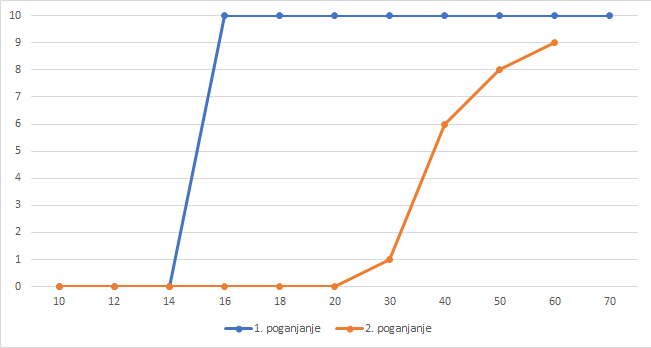
\includegraphics[width=\linewidth]{stevilo_nepravilnih.png}
  \caption{Število nepravilno pobarvanih grafov}
  \label{fig:število nepravilno pobarvanih grafov}
\end{figure}

Slika 1 prikazuje število nepravilno pobarvanih grafov s funkcijo pred in po izboljšavah. Vidimo, da nobena od funkcij do 14 vozlišč ni imela težav, le-te pa so se začele pred izboljšavami pojavljati že pri 16 vozliščih, kjer algoritem ni znal pravilno pobarvati nobenega grafa. Izboljšana funkcija pa je bila v vseh primerih uspešna vse do 20 vozlišč in tudi na več vozliščih je bila veliko boljša od prejšnje.

Prvi graf ki ga funkcija ni uspela pravilno pobarvati je bil na 30 vozliščih, zato sva ga dodala na seznam potencialnih protiprimerov, prikazan je na sliki 2. Potem je s številom vozlišč  število neuspešno pobarvanih grafov strmo narastlo, kar bi lahko pomenilo, da nekaj grafov ni mogoče lokalno iregularno pobarvati s 3 barvami, možno pa je tudi, da je to mogoče vendar bi potrebovali zelo veliko časa ali nekoliko boljši algoritem.

\begin{figure}[H]
  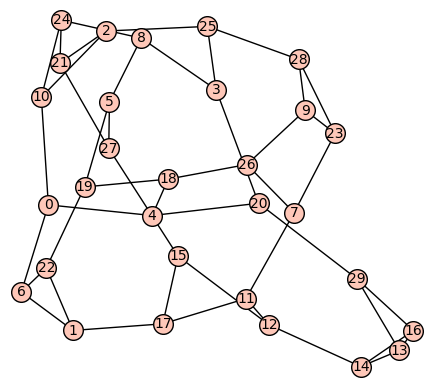
\includegraphics[width=\linewidth]{30_proti.png}
  \caption{Graf na 30 vozliščih, ki ga prvič izboljšana funkcija ni uspela pobarvati}
  \label{fig:Graf na 30 vozliščih, ki ga izboljšana funkcija ni uspela pobarvati}
\end{figure}


\section{Drugo izboljšanje funkcije}

Funkcijo sva spremenila tako, da je število, korakov, namesto fiksnih 3000, odvisno od števila vozlišč v grafu. To sva uporabila le za velike grafe, saj se le tu še pojavljajo težave, število naključnih grafov, pa sva iz 10 zmanjšala na 5. Poleg tega sva s tako spremenjeno funkcijo poizkusila pravilno pobarvati še grafe, ki nama jih prej ni uspelo.

\subsection{Ugotovitve po drugem izboljšanju}

S to funkcijo, sva uspela pravilno pobarvati vse grafe na vozliščih od 14 do 20. Težava se je pojavila pri grafu s 30 vozlišči, kjer eden od grafov ni bil uspešno pobarvan, je pa funkcija tokrat pravilno uspela pobarvati prejšnji graf na 30 vozličih, ki torej ne predstavlja potencialnega protiprimera.


\section{Zaključek}
Algoritem, ki sva ga napisala je za manjše grafe precej uspešen, za grafe na vozliščih od 30 naprej pa deluje nekoliko slabše. Njegova uspešnost je po najinih ugotovitvah precej odvisna od začetnega naključnega barvanja grafa. Zdi se nama, da bi ob z zadostnim številom poskusov barvanja grafov uspeli pobarvati večino na 30 vozliščih, kasneje pa se res lahko pojavijo težavem kot kažejo najini potencialni protiprimeri, ki jih je na grafih z veliko vozlišči kar precej.





\end{document}
